% Sección del artículo — dueño: P4.
\subsection{Líneas base}
Todas las líneas base usan la misma interfaz de controlador y las mismas observaciones que el
dron (nunca la información privilegiada del experto): \emph{directo} (vuela en línea recta
hacia el objetivo), \emph{campos de potencial}~\cite{khatib1986} (atracción al objetivo y
repulsión de los rayos), \emph{A*}~\cite{hart1968} con replanificación sobre el mapa previo
actualizado con los rayos, \emph{A* + ALV}, que al perder el GPS vuelve con el vector
promedio de hitos~\cite{lambrinos2000}, y \emph{A* + supervisor}. Sin GPS todas estiman su
posición integrando brújula y odometría (Fig.~\ref{fig:lineasbase}).

\begin{figure}[t]
\centering
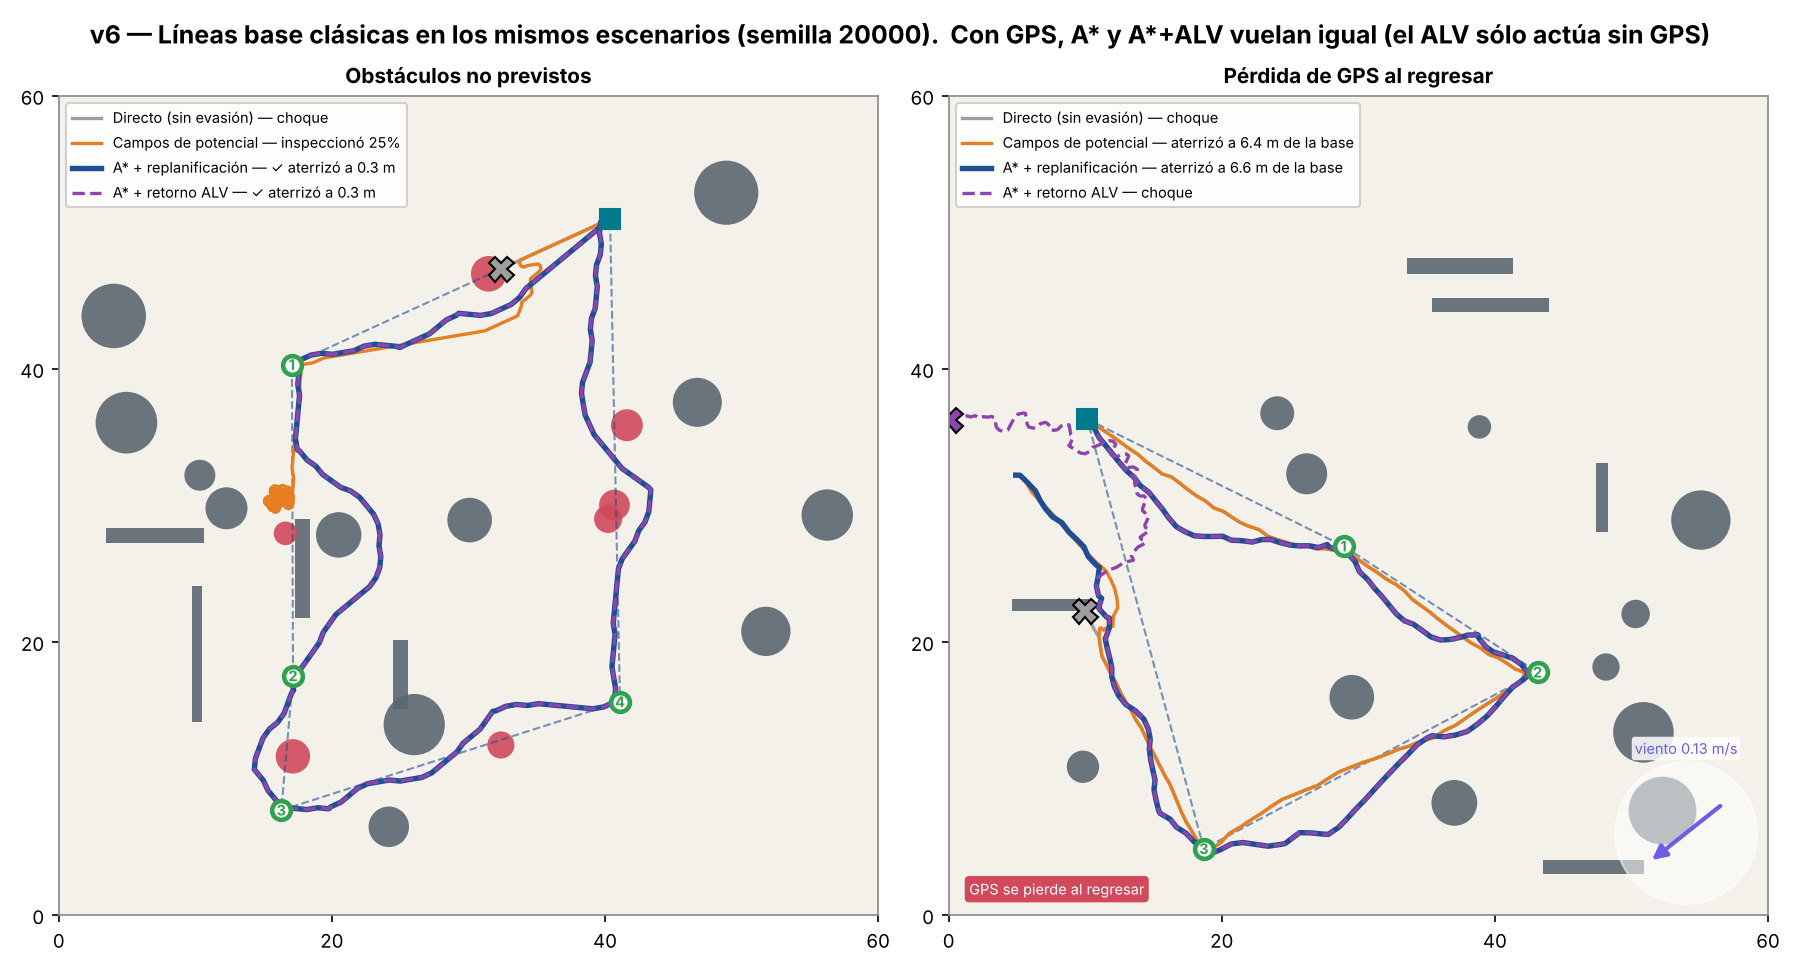
\includegraphics[width=\linewidth]{v6_lineas_base}
\caption{Líneas base en un mismo escenario. Sin GPS, la deriva hace que aterricen lejos de la
base o choquen.}
\label{fig:lineasbase}
\end{figure}
